\documentclass{beamer}

% This file is a solution template for:

% - Talk at a conference/colloquium.
% - Talk length is about 20min.
% - Style is ornate.


\mode<presentation>
{
  \usetheme{Singapore}
  % or ...

  \setbeamercovered{transparent}
  % or whatever (possibly just delete it)
}


\usepackage[utf8]{inputenc}
\usepackage[english]{babel}
\usepackage{textcomp}

% \usepackage{times}
% \usepackage[T1]{fontenc}
% Or whatever. Note that the encoding and the font should match. If T1
% does not look nice, try deleting the line with the fontenc.

\usepackage{graphicx}
\usepackage{epstopdf}
\usepackage{amsmath}
\usepackage{amsfonts}
\usepackage{mathtools}
\usepackage{dsfont}
\usepackage{color}
\usepackage{verbatim}
\usepackage{tikz}
\usepackage{cite}

\title{Plasmonic Properties of QM 2D Fractals.}

\author{Tom Westerhout \\ 
        \emph{Supervisors:} Shengjun Yuan \& Edo van Veen \\
        TCM}
\titlegraphic{\vspace{-2.0cm}\begin{center}\input{Eigenstates-Intro}\end{center}}
\date{}

\begin{document}

\begin{frame}
    \titlepage
\end{frame}

\section{Introduction}

\subsection{Plasmons}

\begin{frame}{Stained Glass}
    \begin{figure}
    \includegraphics[width=8cm]{stained-glass-bird}
    \end{figure}
\end{frame}

\begin{frame}{Plasmons}
    \begin{definition}[Plasmon]
        Quantum of plasma oscillation (\emph{think quasiparticle}).
    \end{definition}

    \begin{definition}[Plasma Oscillation]
        Longitudinal wave of electron charge-density.
    \end{definition}
\end{frame}

\subsection{Fractals}

\begin{frame}{Fractals}
    \begin{itemize}
    \item Features: nowhere differentiable, have fractal dimensions, self-similar, etc.
    \item Ramification: minimum number of links that one needs to remove to separate a macroscopic part of infinite fractal.
        \begin{columns}[T]
        \column{0.6\textwidth}
            \emph{Finite ramification:} \alert{Solved analytically} \\ by L.P. Kadanoff (1982).
        \column{0.4\textwidth}
            \begin{figure}
            \input{Sierpinski-Gasket}
            \end{figure}
        \end{columns}

        \begin{columns}[T]
        \column{0.6\textwidth}
            \emph{Infinite ramification:} \alert{Unsolvable analytically} (?). Numerical calculations exist (\emph{done at Radboud}), but not of plasmonic properties.
        \column{0.4\textwidth}
            \begin{figure}
            \input{Sierpinski-Carpet}
            \end{figure}
        \end{columns}
    \end{itemize}
\end{frame}

\subsection{Physical Description}

\begin{frame}{Tight Binding}
    \begin{columns}[T]
    \column[t]{0.6\textwidth}
        \begin{itemize}
        \item \alert{atomic basis $\{|a\rangle\}$}
        \item Hamiltonian of the system is
            \[ \hat{\mathcal{H}} = -t \,\sum_{\langle a, b \rangle} (\hat c_a^\dagger \hat c_b + \text{h.c.})\;,\]
            $\hat c^\dagger_a$ and $\hat c_a$ are creation and annihilation operators, $t$ is the \alert{hopping} value.
        \item Hopping: 
            \vspace{-0.5cm}
            \[ \underbrace{\hat{c}_a^\dagger \underbrace{\hat c_b |\psi \rangle}_{\mathclap{\text{``take'' from $b$}}}}_{\mathclap{\text{``move'' to $a$}}} \]
        \end{itemize}

    \column[t]{0.4\textwidth}
        \begin{figure}
        \includegraphics[width=\textwidth]{{nearest_neighbours}.pdf}
        \end{figure}
    \end{columns}
\end{frame}

\begin{frame}{System}
    \begin{itemize}
    \item Electron system is described (in one-particle approximation) by
        \begin{itemize}
        \item \alert{eigenenergies $\{E_i\}$} and
        \item \alert{eigenstates $\{|i\rangle\}$}.
        \end{itemize}
    \item Grand-canonical ensemble, i.e. \alert{temperature} $T$ and \alert{chemical potential} $\mu$ are fixed.
    \item Occupational numbers are given by the \alert{Fermi-Dirac distribution}.
    \end{itemize}
\end{frame}

\begin{frame}{Problem}
    \begin{itemize}
    \item All plasmonic properties are obtained from the \alert{dielectric function} $\hat\varepsilon$. \\
        $\implies$ Goal: \alert{calculate $\hat\varepsilon$}.
    \item There exist good methods for calculation of the dielectric function in \alert{momentum space}, i.e. they rely on translational symmetry of the system.
    \item But in fractals, there is \alert{no translational symmetry}!
    \item Calculations have to be done in \alert{real space}. \\
        $\implies$ \alert{New method}.
    \end{itemize}
\end{frame}

\section{Method}

\subsection{Theory}

\begin{frame}{Dielectric Function in Real Space}

    Within the Random Phase Approximation (RPA) we obtain:

    \[ \langle \mathbf{r} | \hat V_\text{ext}(\omega) | \mathbf{r} \rangle = \int\!\! \text{d}^3 r' \; \langle \mathbf{r} | \hat \varepsilon(\omega) | \mathbf{r'} \rangle \langle \mathbf{r'} | \hat V | \mathbf{r'} \rangle \; , \text{ where} 
    \]
    \begin{multline*}
        \langle \mathbf{r} | \hat \varepsilon(\omega) | \mathbf{r'} \rangle 
            = \langle \mathbf{r} | \mathbf{r'} \rangle - \lim_{\eta \to 0+} \sum_{i,\,j} \frac{n_i - n_j}{E_i \!-\! E_j - \hbar(\omega \!+\! i\eta)} \int\!\! \text{d}^3 r'' \frac{e^2}{\| \mathbf{r} - \mathbf{r''} \|} \\
        \times \langle j |\mathbf{r''}\rangle \langle\mathbf{r''} | i \rangle \langle i | \mathbf{r'}\rangle \langle \mathbf{r'} | j \rangle \;.
    \end{multline*}
\end{frame}

\subsection{Implementation}

\begin{frame}{Algorithm}
    Calculating $\hat\varepsilon$ for a single $\omega$ is an \alert{$\mathcal{O}(N^4)$ problem}, where $N$ is the number of particles.
    \begin{itemize}
    \item Hack: rewrite everything in terms of \alert{matrix operations} and use BLAS (\emph{Basic Linear Algebra Subroutines}).
    \item Use a \alert{supercomputer} for calculations.
    \item Hack: use \alert{symmetries} of the system.
    \end{itemize}
\end{frame}


\begin{frame}{Code}
    \begin{itemize}
    \item Written \texttt{C++} package to calculate $\hat\varepsilon$ for a \alert{general} system described by TB.
    \item \alert{$\approx 8.5$ thousands} lines of code (\emph{excluding} data analysis scripts).
    \item $\approx 400000$ computational hours spent, that is \\ \alert{$\approx 45$ years of calculations}.
    \end{itemize}
\end{frame}

\section{Results}

\subsection{Experiments}

\begin{frame}{Electron Energy Loss Spectroscopy (EELS)}
    \begin{columns}[T]
    \column[t]{0.6\textwidth}
        \begin{itemize}
        \item Shoot electrons on the sample.
            \begin{itemize}
            \item Electron beam with a well-defined four-momentum $p^{\mu}$.
            \item Inelastic scattering results in \alert{energy loss $E = \hbar\omega$} and \alert{momentum transfer $\hbar\mathbf{q}$}.
            \end{itemize}
        \item Look at (usually) transmitted electrons.
            \[ \overbrace{\frac{\text{d}^2\sigma}{\text{d}\Omega\text{d}E}} ^{\mathclap{\text{\parbox[c]{3cm}{\normalsize double-differential \\ cross section}}}} \propto\; 
               \underbrace{-\operatorname{Im}\! \left[\frac{1}{\langle\mathbf{q}| \hat\varepsilon(\omega) |\mathbf{q}\rangle}\right]} _\text{\normalsize \alert{loss function}} \;.
            \] %
        \end{itemize}
    \column[t]{0.4\textwidth}
        \vspace{-0.3cm}
        \begin{figure}
        \includegraphics[height=6.5cm]{EELS-crop.pdf}
        \end{figure}
    \end{columns}
\end{frame}

\subsection{Calculations}

\begin{frame}{Third Iteration Sierpinski Carpet}{System}
    \begin{figure}
    \vspace{-.5cm}
    \input{Coordinates-SC-3}
    \end{figure}
\end{frame}

\begin{frame}{Third Iteration Sierpinski Carpet}{Results}
    \begin{figure}
    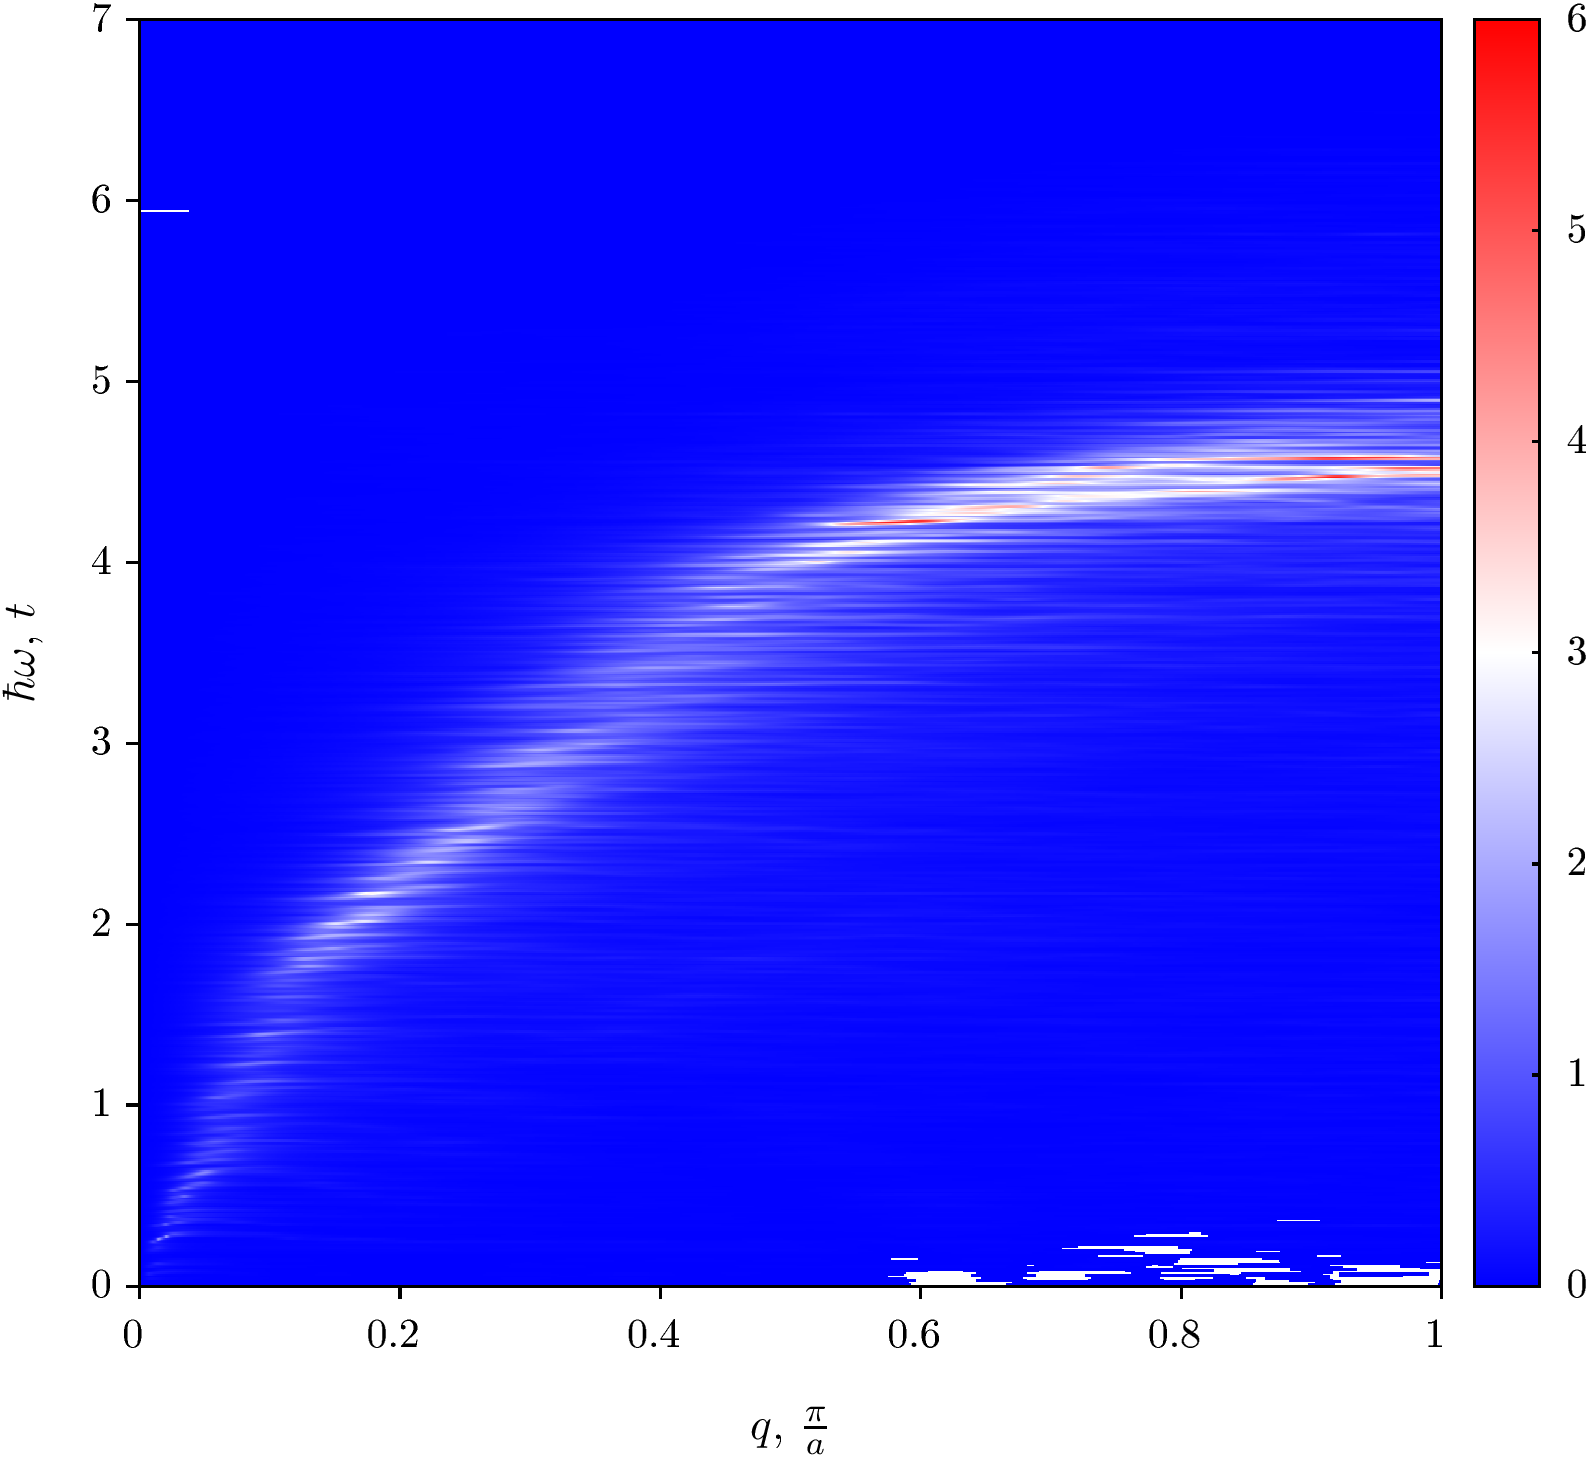
\includegraphics{Spectrum-3rd-Q-Omega}
    \end{figure}
\end{frame}

\begin{frame}{Square Lattice}{Results}
    \begin{figure}
    \includegraphics{Spectrum-3rd-SL-Q-Omega}
    \end{figure}
\end{frame}



\section{Summary}

\begin{frame}{Summary}
  \begin{itemize}
  \item \Large{It \emph{is} possible to do calculations of $\hat\varepsilon$ in real space.}
  \item \Large{There \emph{are} well defined plasmons in Sierpinski carpets, which is \emph{unexpected} for a system without translational invariance.}
  \item \Large{The created package can be \emph{reused} to study plasmonic properties of other systems.}
  \end{itemize}
\end{frame}

\begin{frame}{Outlook}
    \begin{itemize}
    \item \Large{Publish the results, i.e. write a paper.}
    \item \Large{Look at \emph{other} systems with no translational symmetry.}
    \end{itemize}
\end{frame}

\begin{frame}{}
    \vfill
    \begin{minipage}{\textwidth}
    \begin{center}
        \Large Any questions?
    \end{center}
    \end{minipage}
    \vfill
\end{frame}


% All of the following is optional and typically not needed. 
\appendix

\section{For Extra Information}

\begin{frame}{Simple example of plasma oscillation}
    \begin{itemize}
    \item Free electron gas with positively charged atom cores in the background.
    \item Oscillating electric field $\mathbf{E}(t) = \mathbf{E_0}\exp(-i\omega t)$.
    \item Equation of motion: \[ \mathbf{\ddot{x}} + \gamma\mathbf{\dot{x}} = -\frac{e}{m}\mathbf{E}(t)\; .\]
    \item Displaced electrons generate a polarization $\mathbf{P} = -Ne\mathbf{x}$ \\ ($N$ is the electron density).
    \item From $\epsilon_0\mathbf{E} + \mathbf{P} = \epsilon_0\varepsilon(\omega)\mathbf{E}$ \ we get $\varepsilon(\omega)$.
    \item In high frequency limit $\varepsilon(\omega) \approx 1 - \frac{\omega_p^2}{\omega^2}$, \\ $\omega_p$ --- \alert{plasma frequency}.
    \item If $\omega = \omega_p$, we get longitudinal oscillation of electron-charge density.
    \end{itemize}
\end{frame}

\begin{frame}{Random Phase Approximation}
    \begin{itemize}
    \item Perturbation of the form
        \[ \alert{\hat V e^{-i(\omega + i\eta)t}}\,,\text{ with }\eta \to +0\,. \]
        \small{($\hat V$ is diagonal in $\mathbf{r}$-basis, i.e. $\langle\mathbf{r}|\hat V|\mathbf{r'}\rangle = V(\mathbf{r})\delta^3(\mathbf{r} - \mathbf{r'})$)}
    \item Results in an induced charge density variation $\delta\hat N(t)$
    \item \alert{Self-consistency equation}
        \[ \langle \mathbf{r} | \hat V_\text{tot}(t) | \mathbf{r} \rangle
            = \langle \mathbf{r} | \hat V_\text{ext}(t) | \mathbf{r} \rangle + \int\!\! \text{d}^3 r' \; \langle \mathbf{r} | \hat V_\text{Coulomb} | \mathbf{r'} \rangle \langle \mathbf{r'} | \delta\hat N(t) | \mathbf{r'} \rangle \;. \]
    \end{itemize}
\end{frame}

\end{document}



